\section{Simulations and Tests}
Vanet Simulator is written in Java because this programming language is really powerful and flexible to use but more over we see the Java problems with cryptography. First of all the Java security implementation, at this time (version 1.6.x), do not include elliptic curves for asymmetric cryptography and we have research on internet a provider which release elliptic curves and we have found \textit{Bouncy Castle}\footnote{See bibliography at \pageref{bibliography} for more details on this provider}, after this step we have choosen the security level of digital signature and we have opted for 163 bit of \textit{nistb} curves, the less security level in this cryptography provider, after that we have compute with \emph{openssl}\footnote{See bibliography at page \pageref{bibliography} for more details} the tipical speed\footnote{For computation we have used: Pentium 4 Core 2 Duo, processor: Intel T5450 (1.66GHz, 667 Mhz FSB, 2 MB L2 Cache, 2 GB DDR2 RAM} for sign and verify a digital message, see table \ref{tab:OpensslVelocity} at page \pageref{tab:OpensslVelocity}.
\begin{table}[!ht]
	\centering
	\caption{OpenSSL Speed Analysis}
	\begin{tabular}{|c|c|c|c|}
	\hline\hline 
	\textbf{Sign} & \textbf{Verify} & \textbf{sign/s} & \textbf{verify/s} \\
	\hline
	0.0017s & 0.0050s & 583.5 & 199.3 \\
	\hline
	\hline     %inserts single line 
 	\end{tabular} 
	\label{tab:OpensslVelocity}
\end{table}
The Bouncy Castle implementation is slowly than OpenSLL and we have found on time order of difference between C (OpenSSL)  implementation and Java implementation (Bouncy Castle), see table \ref{tab:BouncyCastleVelocity} at page \pageref{tab:BouncyCastleVelocity}.
\begin{table}[!ht]
	\centering
	\caption{Bouncy Castle Speed Analysis}
	\begin{tabular}{|c|c|c|c|}
	\hline\hline 
	\textbf{Sign} & \textbf{Verify} & \textbf{sign/s} & \textbf{verify/s} \\
	\hline
	0.028031s & 0.017342s & 35.6 & 57.6 \\
	\hline
	\hline     %inserts single line 
 	\end{tabular} 
	\label{tab:BouncyCastleVelocity}
\end{table}
In additional analysis we have to verify the certificates with the certification authority and for do that in Java we spent tipically $0.038708s$ roughly $25.83 {verify \over s}$
\subsection{Criptography Overhead}\label{sec:CryptographyOverhead}
In this section we want spent two words around cryptography overhead. During simulation we sent 200 bytes of payload but this payload is securized and for do that we have to insert more bytes for signature and certificate for realize digital signatures. These attachements increase the packet dimensions and for that reason is really useful use optimizations \cite{calandriello}, see table \ref{tab:CryptographyOverhead} at page \pageref{tab:CryptographyOverhead} for more details.
\begin{table}[!ht]
	\centering
	\caption{Cripography Overhead}
	\begin{tabular}{|c|c|}
	\hline\hline 
	\textbf{Signature} & \textbf{Certificate}\\
	\hline
		48 & 234\\
	\hline
	\hline     %inserts single line 
 	\end{tabular} 
	\label{tab:CryptographyOverhead}
\end{table}
\subsection{Real Vanet implementation to Simulator}
Before see the simulation of Vanet, we have to underline the difference between real vanet implementation to simulator. The main task of Vehicular Networks is privacy, integrity and not repudiation of messages and for do that we use a lot of methods, like pseudonyms change or group keys. In the simulator we are obliged to use all network stack from application level to physical level and this feature remove privacy because we are not able to change MAC address dinamically and if we analize the network traffic we can found MAC address and track vehicle moves. Real system do not use the complete network stack and work only on level two (MAC layer) with changing MAC address for every beacon sent on the network.
\subsection{Simulation of Baseline Pseudonyms}
Before starting simulations in baseline psedonyms you have to modify the configuration file \textit{base.properties} \footnote{See the user manual for more information around configurations. Section \ref{usermanual:baseconfiguration} at page \pageref{usermanual:baseconfiguration}} under folder \textit{properties} in root directory of Vanet Simulator.\\
For \baseline we can realize three different optimizations picked up from \cite{calandriello} but in this simulator we have realized the second optimization, in particular the sender append \textit{beacon identification}, \textit{signature}, \textit{public key} and \textit{certificate} only for $\alpha$ messages and transmitt only \textit{beacon identification} and \textit{signature} for remaining $\alpha-1$ beacons. \\
The beacon identification is random number compute on four byte without consider other vehicles, is resonable to use this method whitout remember other IDs is because probability which two vehicle use the same identification number is really quite.
\baseline use optimization two from \cite{calandriello} for limit cryptography overhead, see section \ref{sec:CryptographyOverhead} at page \pageref{sec:CryptographyOverhead} for importance of cryptography overhead, and you can change parameters for realize you personal optimization, for example certificate reattach after tot beacons and certificate or change certificate after a period of time.
\subsection{Performance of Simulator}
For analyze performace of Simulator (figure \ref{fig:performance} at page \pageref{fig:performance}) we have computed statistics for understand the number of signature which we are able to do with the simulator. We have set up the \baseline simulator and set logger into console, after that we have ran system and observed comportaments modifing the number of beacons/sec and the number of vehicles into wireless area.
\begin{figure}[ht]
% If the picture uses fonts of the correct size (10 ... 12 pt)
% then can be included without scaling
%\centerline{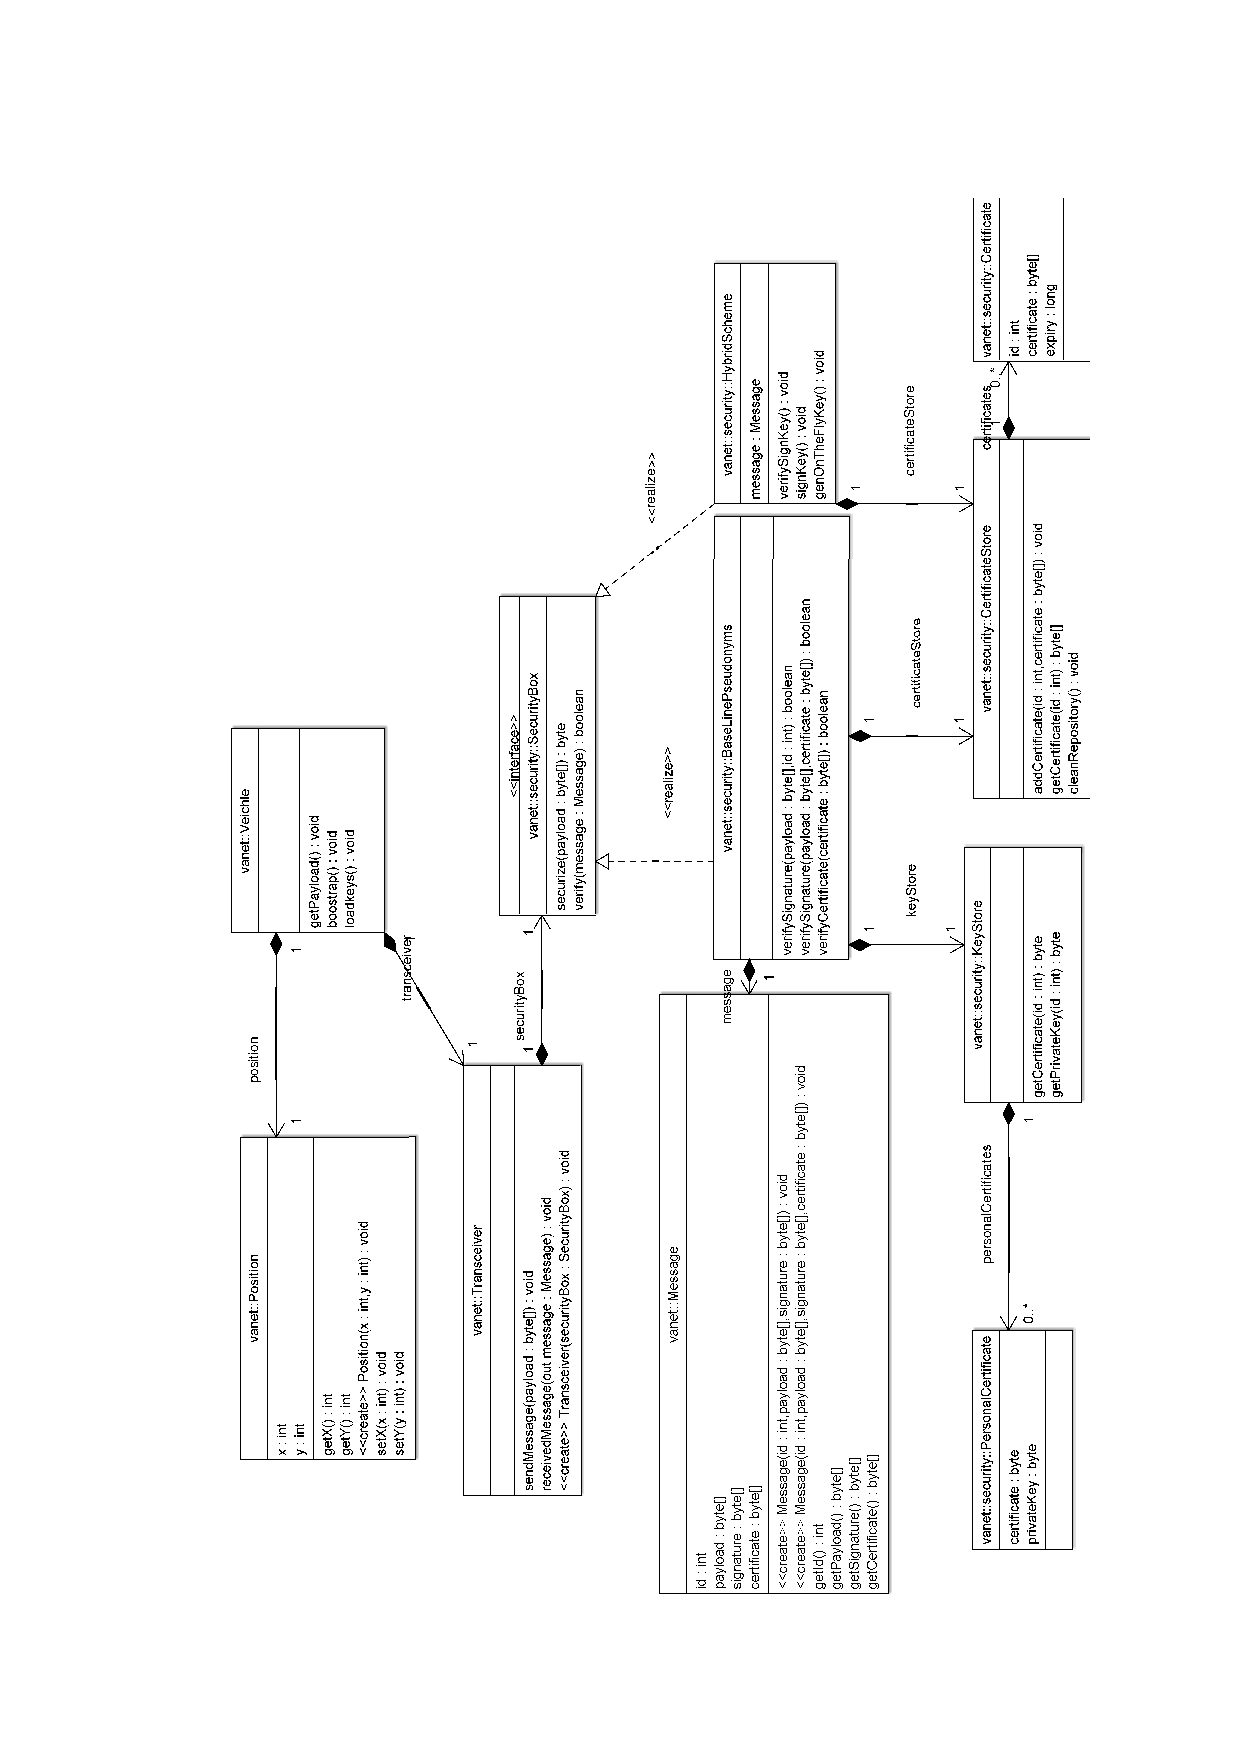
\includegraphics{class_diagram.pdf}}
% otherwise see the example in the following (commented out) line
% to scale it relatively to the page width
\centerline{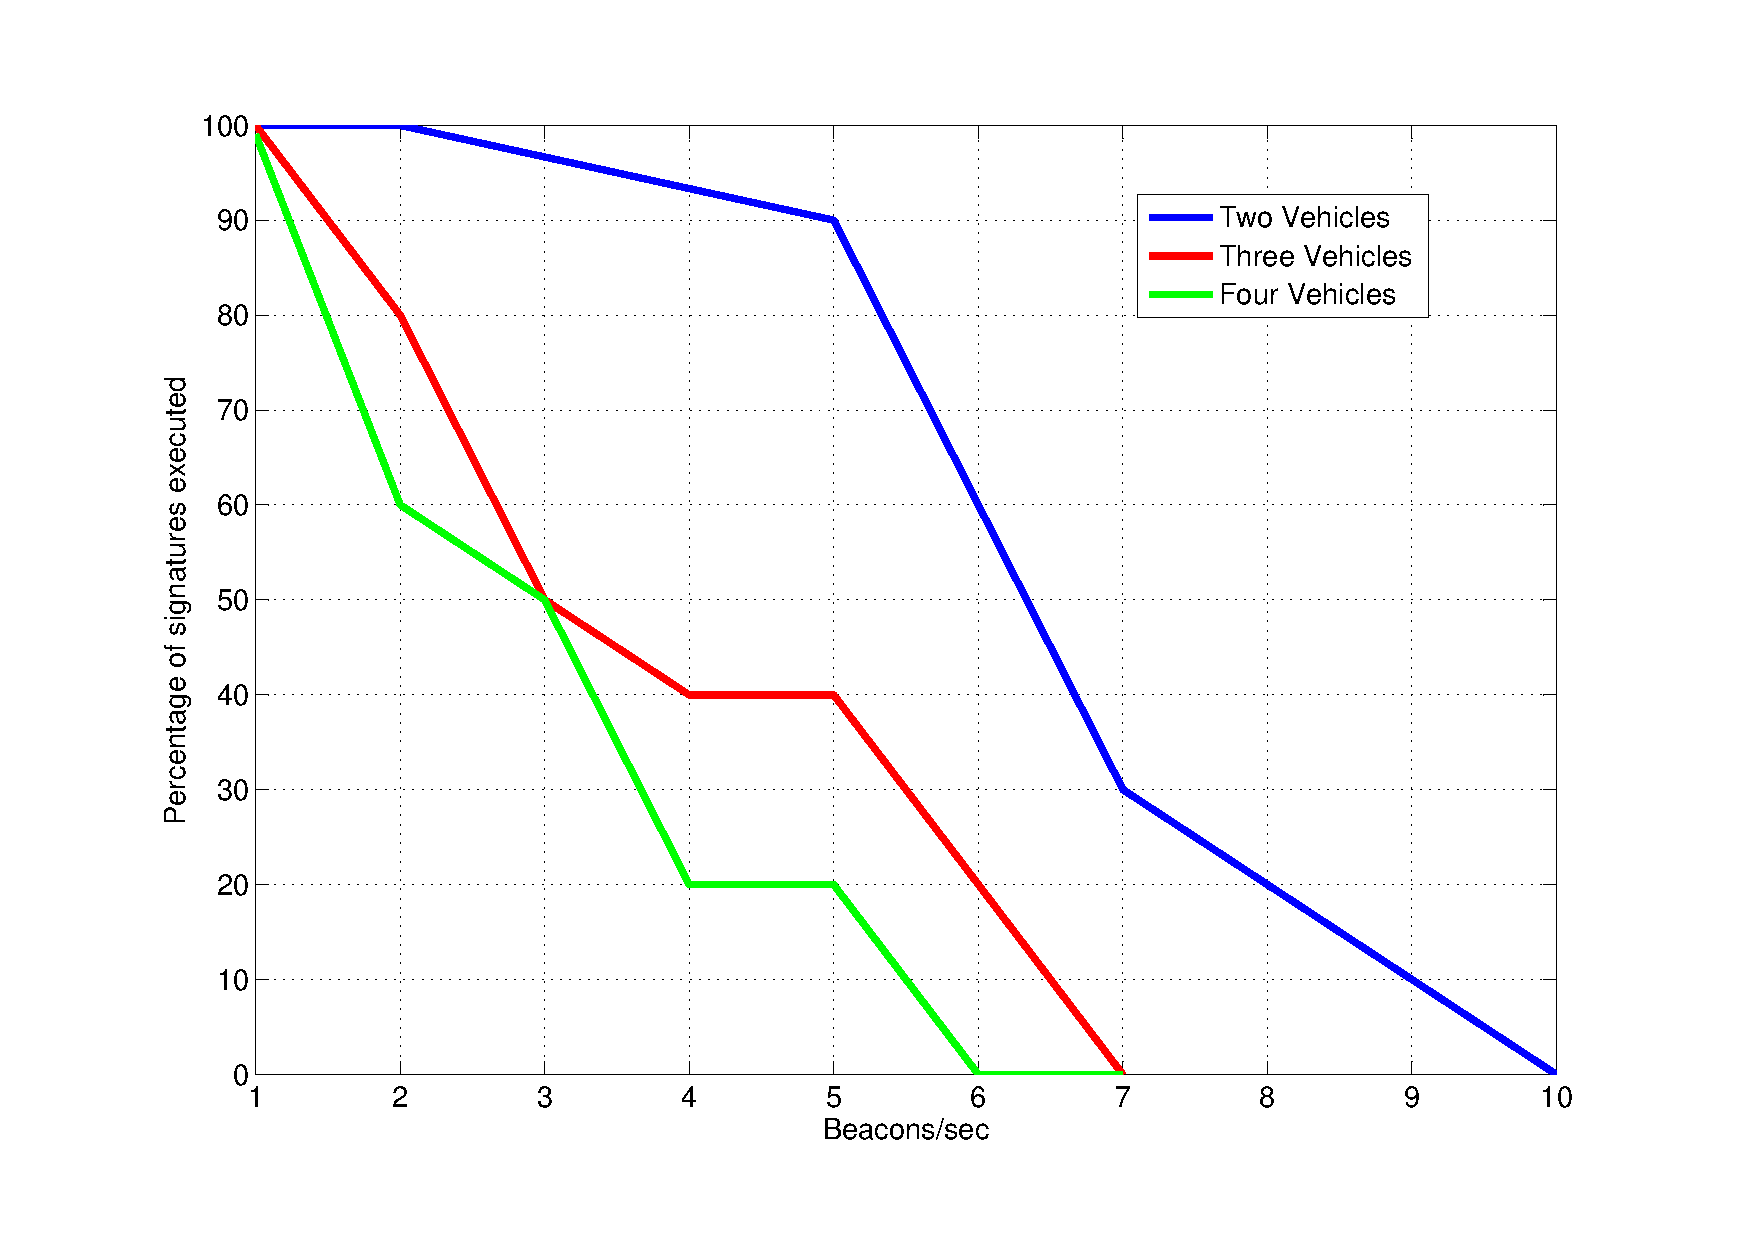
\includegraphics[width=0.5\textwidth]{chart_baseline.pdf}}
\caption{Performace of simulator}
\label{fig:performance}
\end{figure}
